%DIJOUS
\newcommand{\refscreen}[1]{\hyperref[fig:montezuma-map]{screen~#1}}
\chapter{Methodology}
\section{\acl{MR}}
\subsection{Description}
You, the player, are Panama Joe, an intrepid explorer-archaeologist. Your latest
trip has brought you to discover the entrance to an Aztec pyramid. Filled with
excitement, you rush to search the treasures that surely await inside. But the
pyramid is full of traps and monsters. You will need all of your wits and agility to
get out alive!\footnote{Game background from the review by \citet{adair2007montezuma}.}

In the game, Panama Joe can run, jump and climb ladders, ropes and poles. The
pyramid he can explore is divided in 24 screens, numbered 0--23, depicted in
\ffref{fig:montezuma-map}. The player starts the game in screen 1 and ends when
collecting the gems in screen 15. When the player completes the game, it simply
resets with a different colour scheme.

Joe has a number of lives, initially 5. When they are over and Joe loses a life
again, the game is over. Lives can be lost by touching monsters, touching blue
wall traps (such as those in \refscreen{12}), falling
into quicksand pits or falling from too high.

The player can gain score for a number of things: collecting gems (+1000),
keys (+100), the sword (+100), the torch (+3000) or the mallet (+200); opening a
door (+300); or killing a monster with the sword (+2000). A life
is gained for every $10\,000$ points gained, with a maximum of 6 lives. The
torch allows you to see in the lowest floor of the pyramid (which is otherwise
black). The sword allows you to kill one monster. The mallet allows you to be
immune to monsters for a period of time.

The game can be rendered impossible to complete, since there are 6 doors but
only 4 keys. The two doors in \refscreen{17} need to be opened to finish, and
either one of the doors in \refscreen{1} needs to be opened to do almost
anything. So the player can either open both doors in \refscreen{1} and not see
in the bottom floor, or leave one door in each of the screens 1 and 4 unopened.

\begin{figure}[p]
\setlength{\unitlength}{\textwidth}
\begin{center}
%\noindent\makebox[\textwidth]{
  \begin{picture}(1,.513)
    \put(0,0){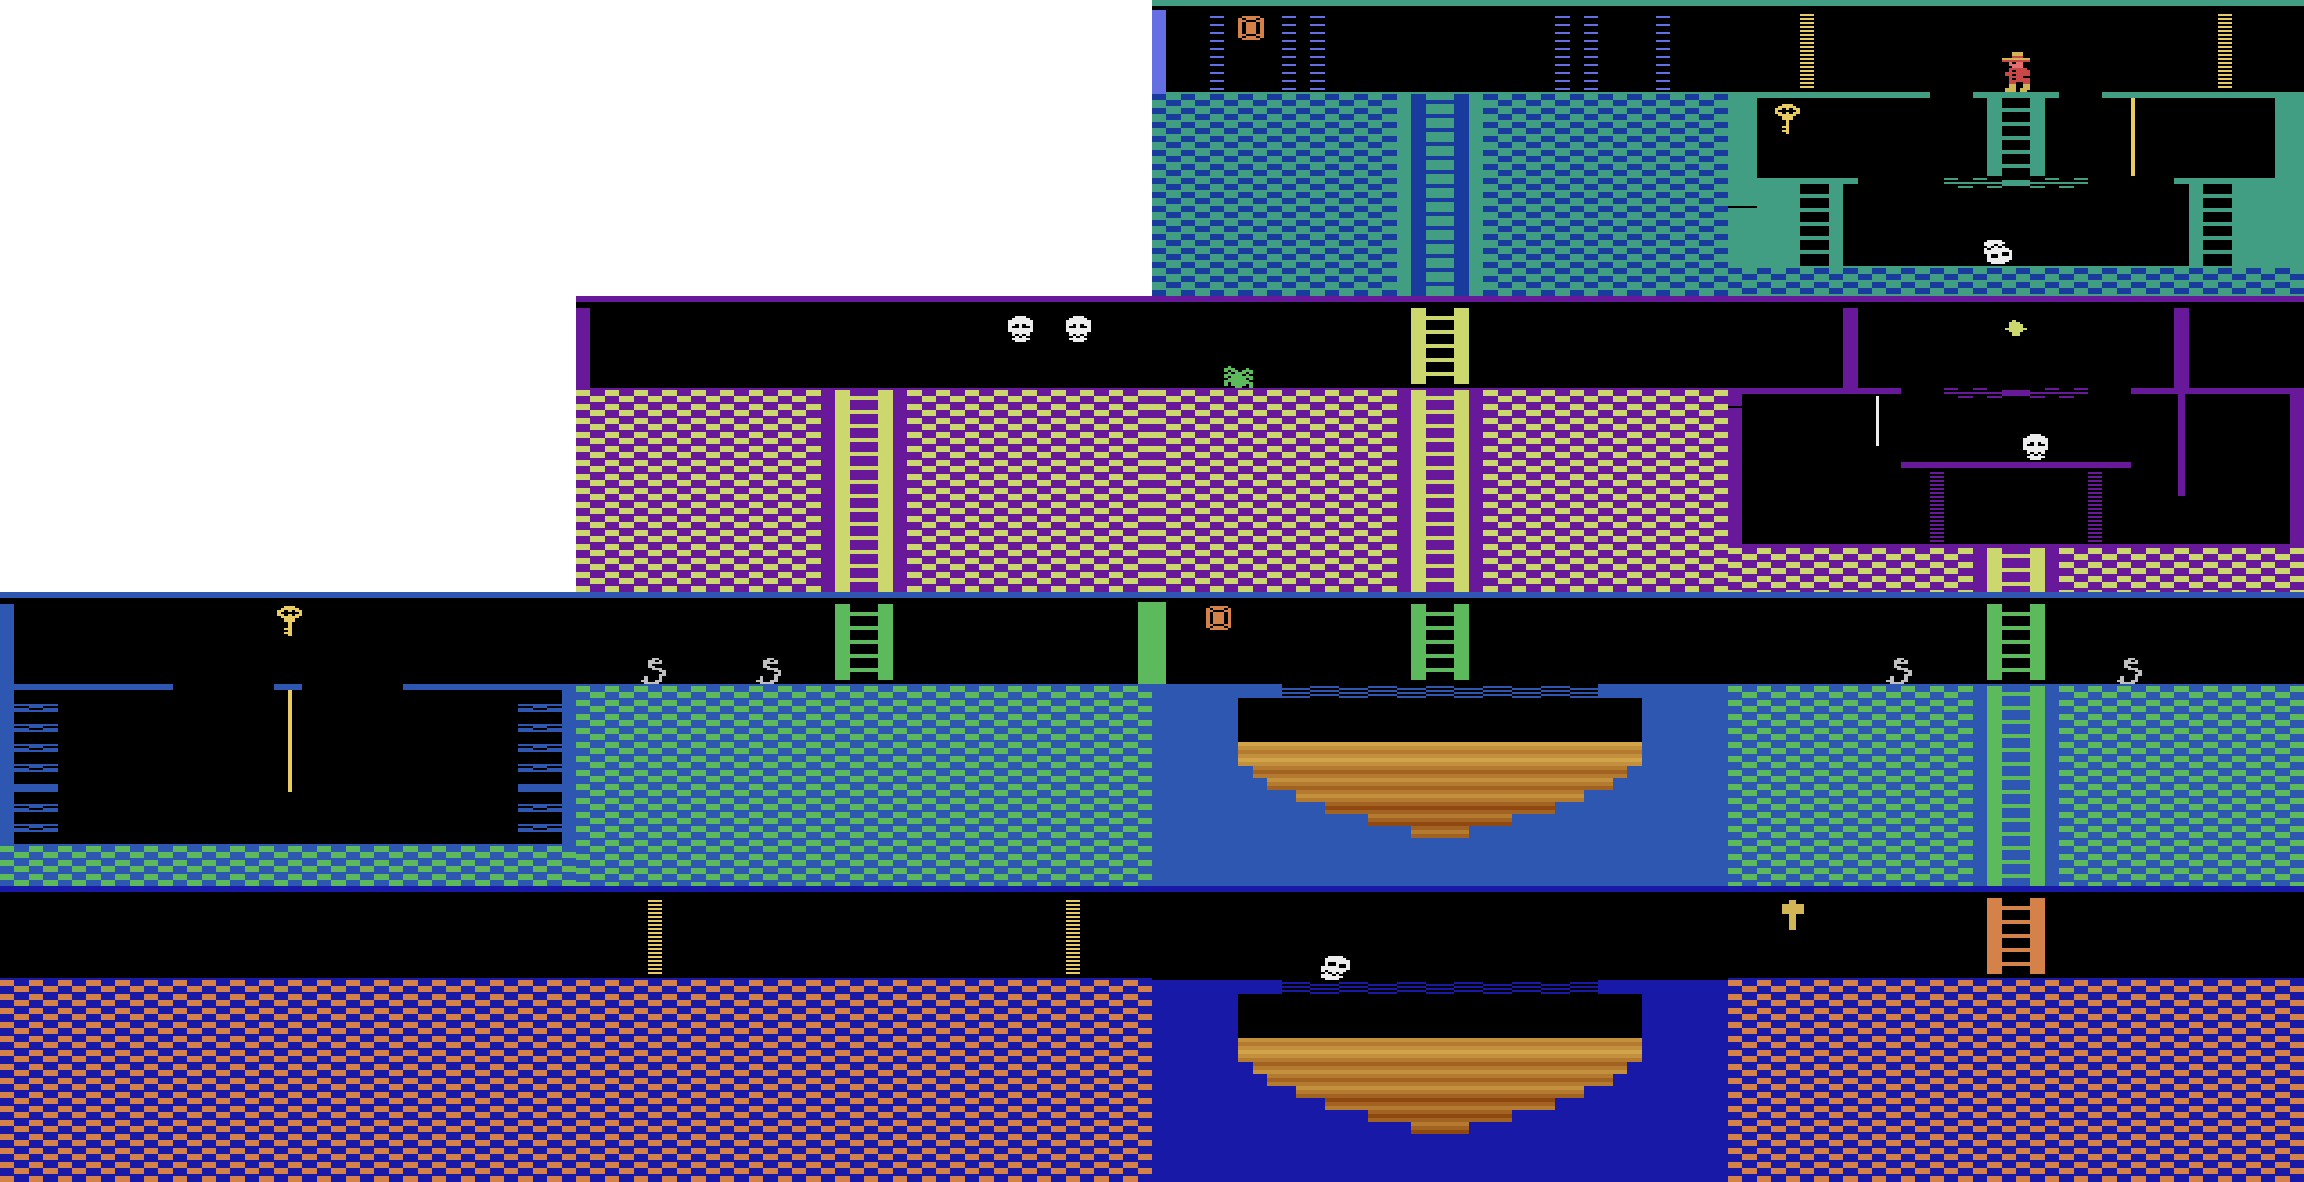
\includegraphics[width=\unitlength]{img/montezuma_all_pt1.png}}
    \put(.58,.485){\color[rgb]{1,1,1}\makebox(0,0)[lb]{0}}
    \put(.83,.485){\color[rgb]{1,1,1}\makebox(0,0)[lb]{1}}
    \put(.33,.357){\color[rgb]{1,1,1}\makebox(0,0)[lb]{3}}
    \put(.58,.357){\color[rgb]{1,1,1}\makebox(0,0)[lb]{4}}
    \put(.83,.357){\color[rgb]{1,1,1}\makebox(0,0)[lb]{5}}
    \put(.08,.228){\color[rgb]{1,1,1}\makebox(0,0)[lb]{8}}
    \put(.30,.228){\color[rgb]{1,1,1}\makebox(0,0)[lb]{9}}
    \put(.58,.228){\color[rgb]{1,1,1}\makebox(0,0)[lb]{10}}
    \put(.83,.228){\color[rgb]{1,1,1}\makebox(0,0)[lb]{11}}
    \put(.08,.1){\color[rgb]{1,1,1}\makebox(0,0)[lb]{16}}
    \put(.33,.1){\color[rgb]{1,1,1}\makebox(0,0)[lb]{17}}
    \put(.6,.1){\color[rgb]{1,1,1}\makebox(0,0)[lb]{18}}
    \put(.83,.1){\color[rgb]{1,1,1}\makebox(0,0)[lb]{19}}
  \end{picture}
%}

\vspace{.2cm}

%\noindent\makebox[\textwidth]{
  \begin{picture}(1,.513)
    \put(0,0){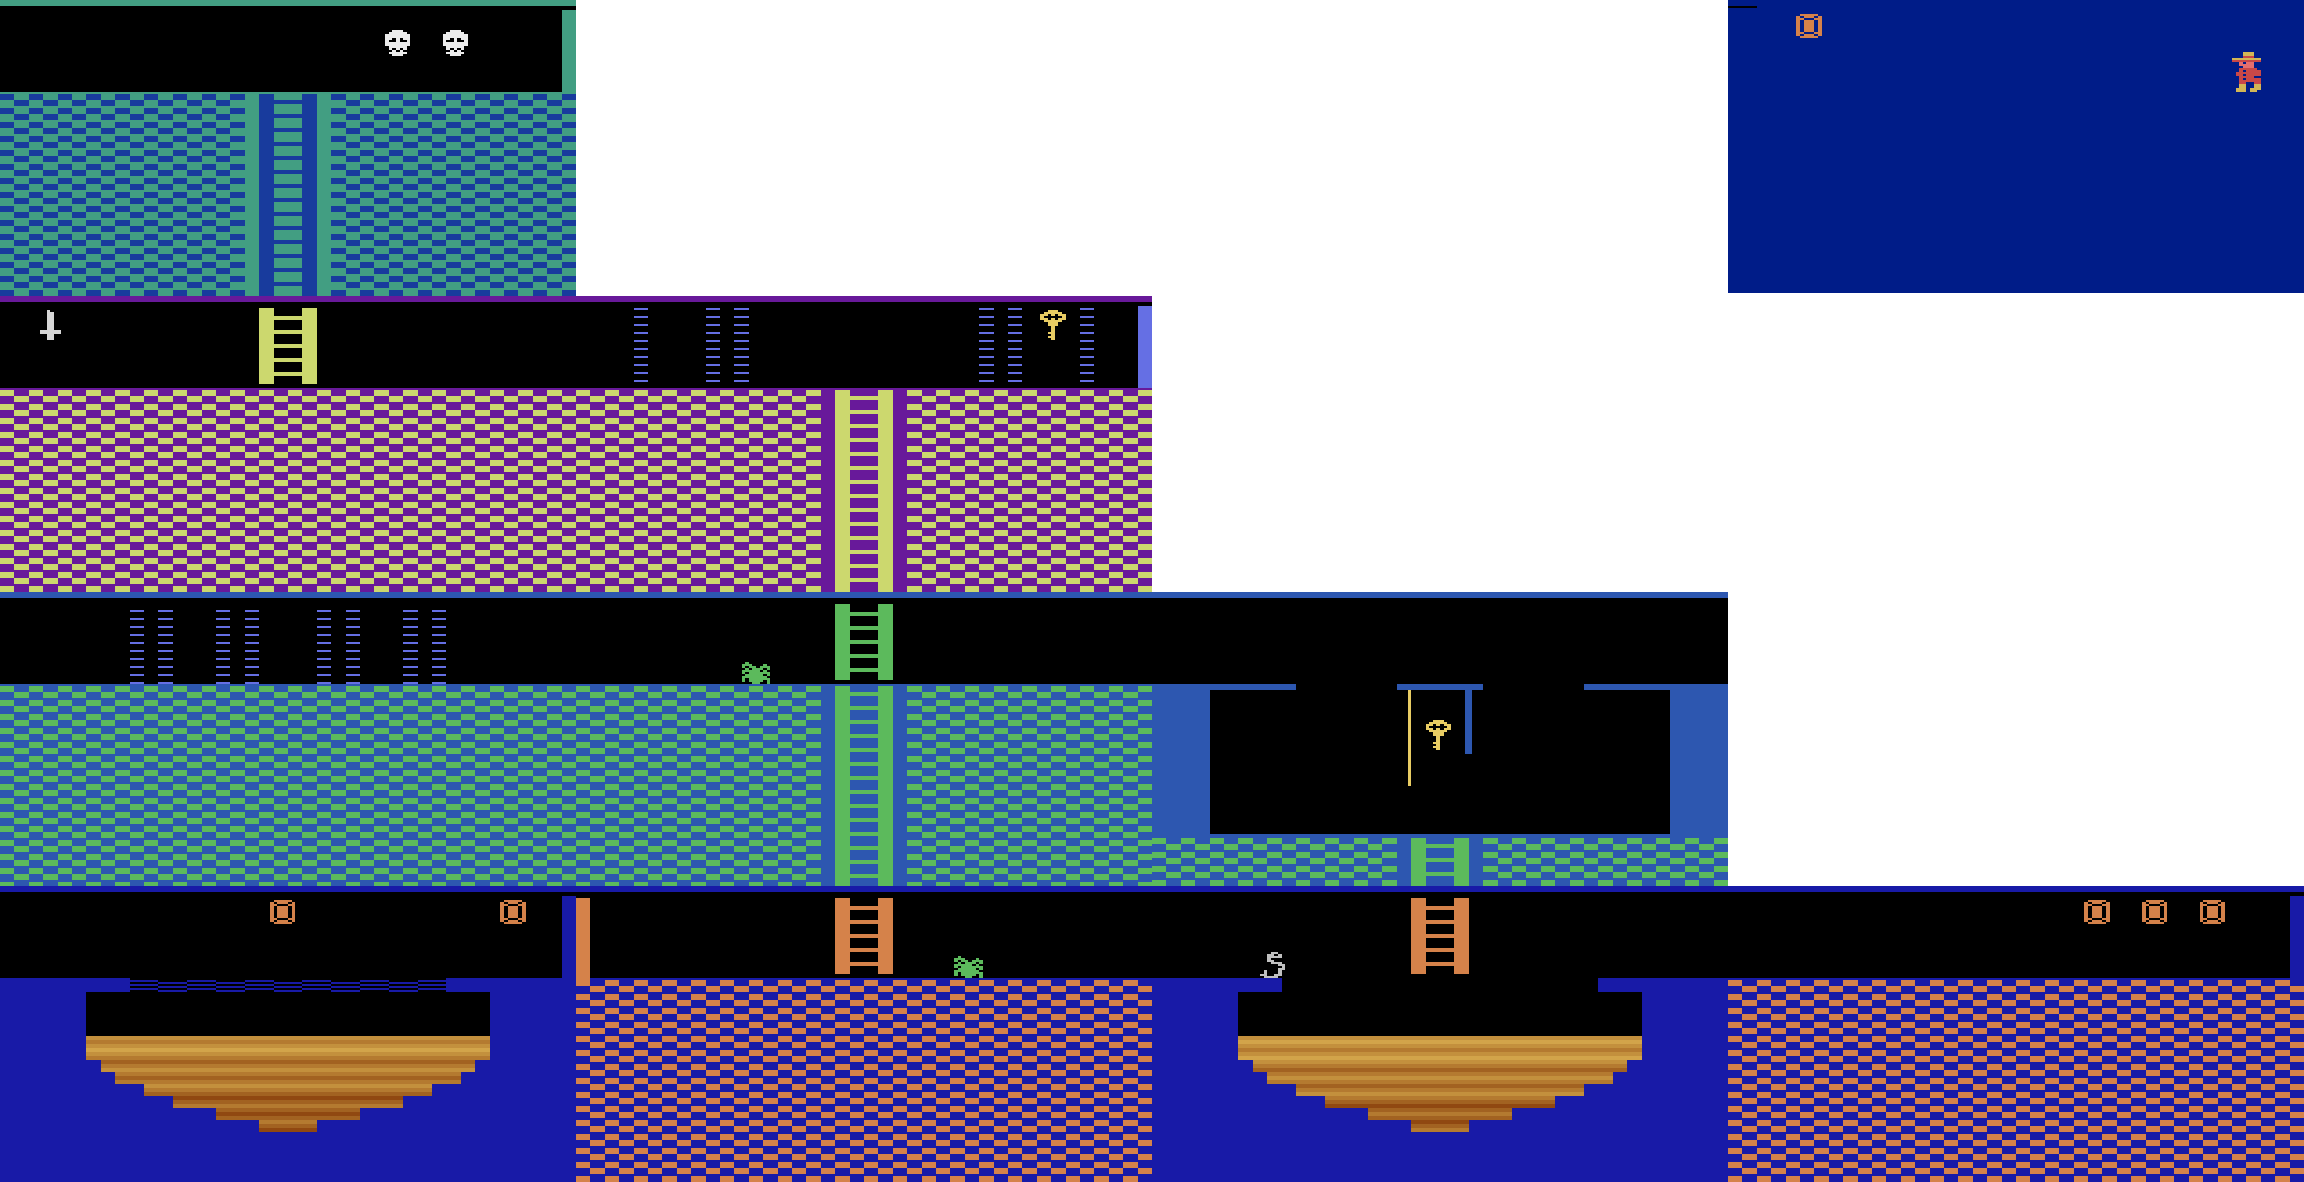
\includegraphics[width=\unitlength]{img/montezuma_all_pt2.png}}
    \put(.08,.485){\color[rgb]{1,1,1}\makebox(0,0)[lb]{2}}
    \put(.83,.485){\color[rgb]{1,1,1}\makebox(0,0)[lb]{15}}
    \put(.08,.357){\color[rgb]{1,1,1}\makebox(0,0)[lb]{6}}
    \put(.33,.357){\color[rgb]{1,1,1}\makebox(0,0)[lb]{7}}
    \put(.04,.228){\color[rgb]{1,1,1}\makebox(0,0)[lb]{12}}
    \put(.28,.228){\color[rgb]{1,1,1}\makebox(0,0)[lb]{13}}
    \put(.58,.228){\color[rgb]{1,1,1}\makebox(0,0)[lb]{14}}
    \put(.08,.1){\color[rgb]{1,1,1}\makebox(0,0)[lb]{20}}
    \put(.33,.1){\color[rgb]{1,1,1}\makebox(0,0)[lb]{21}}
    \put(.58,.1){\color[rgb]{1,1,1}\makebox(0,0)[lb]{22}}
    \put(.83,.1){\color[rgb]{1,1,1}\makebox(0,0)[lb]{23}}
  \end{picture}
%}
\end{center}
\caption[The complete map of \acl{MR}.]{The complete map of \acl{MR}. Rooms are
numbered from left to right and from top to bottom. The pyramid they form has
been cut to fit in the page. Room 15 is located to the left of room 16. The
screens are not numbered in the game. The player starts in room 1 and finishes
in room 15.\label{fig:montezuma-map}}
\end{figure}

\subsection{Reverse-engineering \acl{MR}}
We used the \acl{ALE} (\cite{bellemare2013arcade}) to take several simultaneous
screen and \ac{RAM} snapshots. We usually took 5 to 10 snapshots in the space of
1 or 2 seconds, while performing certain action in the game. Then, we looked at
the bytes that changed value from snapshot to snapshot.

We also used the debugger built-in to the Atari 2600 emulator, Stella
(\cite{stella}). Using the command \verb-breakif <condition>-, that pauses the
game and shows the debugger if a condition is met, enabled us to play and check
whether a memory position behaved as we suspected. In some cases we used the
disassembled code in that debugger too.

In \ffref{tab:atari-ram} and in the list below we reproduce the layout of
the Atari 2600's main memory and what each position affects in \acl{MR}.

Some entries can be modified in the Stella debugger when the game is running,
and affect the game. If an entry is not editable, it will be marked with an
asterisk (*). The values that are not marked editable may be editable in other
circumstances, and are probably editable in the middle of the computations
within a frame. However, their value has been observed only going back to what
it was if modified between frames.

\fxwarning{Explain the Atari's RAM, explain Panama Joe}
\fxwarning{Talk about the RAM of the Atari having 128 bytes and the ones
  relevant are 0x80 0xff. Also about the ROM}
\fxwarning{TAlk about MR.
There seem to be two sprites drawn to screen: one "key" and one "skull", named
after them in the first screen. We will call the first "collectible sprite", but
it can be a monster too}


\begin{table}[hbtp]
\begin{center}
\newcommand{\ram}[2]{\hyperref[ram:#1]{#2*}}
\newcommand{\rame}[2]{\hyperref[ram:#1]{#2}}
%\newcommand{\ram}[2]{\ref{ram:#1}*}
%\newcommand{\rame}[2]{\ref{ram:#1}}
\begin{tabular}{c|cccccccccccccccc}
  & 0 & 1 & 2 & 3 & 4 & 5 & 6 & 7 & 8 & 9 & A & B & C & D & E & F \\
\hline
8 &   &   &   &\rame{screen}{83}&   &   &   &   &   &   &   &   &   &   &   &   \\
9 &   &   &   &\rame{score}{93}& \rame{score}{94}& \rame{score}{95}&   &   &   &   &   &   &   &   &\ram{player-sprite}{9E}&   \\
A &   &   &   &   &   &   &   &   &   &   &\rame{x}{AA}&\rame{y}{AB}&   &   &   &   \\
B &   &\rame{collectable}{B1}&\rame{collectable-colour}{B2}&  &\rame{look-lr}{B4}&  &   &   &   &   &   \rame{lives}{BA} & & & &\rame{skull-animation}{BE}&\rame{skull-jump-y}{BF}\\
C &   &\rame{inventory}{C1}&\ram{doors}{C2}&\rame{skull-moving}{C3}&   &   &   &   &   &   &   &   &   &   &\rame{skull-rotate-y}{AE}&\rame{skull-rotate-x}{AF}\\
D &   &   &   &   &\rame{sprite-modifier}{D4}&   &  \rame{jump}{D6}&   &\rame{fall}{D8}&   &   &   &   &   &  & \\
E &   &   &   &   &   &   &   &   &   &   &\ram{skull-n-rotations}{EA}&   &   &   &   &   \\
F &   &   &   &   &   &   &   &   &   &   &   &   &   &   &   &   \\
\end{tabular}

\end{center}
\caption{The known \acs{RAM} layout for \acl{MR}.\label{tab:atari-ram}}
\end{table}

{
\newcommand{\entry}[2]{\item\label{ram:#1}\textbf{0x#2}: Not editable.}
\newcommand{\entrye}[2]{\item\label{ram:#1}\textbf{0x#2}: Editable.}
\newcommand{\n}[1]{0x#1}

\begin{enumerate}
\entrye{lives}{BA} The number of lives the player has left, that is, the number of
times the player can die and continue the game afterwards. Controls the number
of hats displayed at the top. Panama Joe starts with 5 lives. The counter can go
up to 6 without graphical problems.

\entrye{screen}{83} The current screen. If edited, the new screen will only be
partially drawn. Sometimes, one can exit the screen and reenter it by playing
and the issue will go away.

\entrye{x}{AA} The X position of the character. If set to the middle of the air,
Panama Joe will fall.

\entrye{y}{AB} The Y position of the character. If set to the middle of the air,
and there is a platform below, the character will not fall! Instead, it will
behave as if it was on a ladder. The Y values of the three floors that every
level has are \n{94} or \n{9C}, \n{C0}, and \n{EB}.

\entrye{jump}{D6} The current frame of the jump. Set to \n{FF} when in the
ground. Set to \n{13} when the jump starts. When jumping, the game adds to the Y
of Panama Joe the values from the array starting at memory position \n{E47}.
Thus, if set to higher than \n{13}, the game behaves oddly. It also can be reset
to whatever value at any time, causing Panama Joe to start a jump, even in
mid-air.

\entrye{fall}{D8} The current frame of the fall. Normally set to \n{00}. When falling
off an elevated ground, or off a jump, this value will begin to count up. If it
is \n{08} or higher when Panama Joe touches the ground, he will die.

\item\label{ram:score}\textbf{0x93}, \textbf{0x94}, \textbf{0x95}: Editable. The
score, represented in \acl{BCD}. This is, every nibble represents a decimal digit.

\entrye{inventory}{C1} The contents of the player's inventory. Each possible
object in it is associated to a bit, that is set if the object is in the
inventory. At most 6 objects can be carried without causing graphical
corruptions. The objects and their associations are:
\begin{center}
\begin{tabular}{c|c|c|c|c|c|c|c}
\n{80} & \n{40} & \n{20} & \n{10} & \n{08} & \n{04} & \n{02} & \n{01} \\
\hline
torch & sword & sword & key & key & key & key & mallet \\
\end{tabular}
\end{center}
If the inventory's value is changed, collecting items the normal way stops
working.

\entry{doors}{C2 (bits 3, 2)} Whether the doors in the screen are closed or
open. Only means this in screens 1, 5 and 17. When the bit is set, the door is
closed. Bit 3 controls the door in the left, bit 2 the one in the right.

\entrye{skull-animation}{BE} The frame of the rotating skull's animation, in
screens where there is one.

\entrye{skull-rotate-x}{AF} X of the rotating skull, when there is one (screens
1 and 18). It is not in the same scale as the player's X.
\entrye{skull-rotate-y}{AE} Y of the rotating skull. Also in its own scale, and
cannot take it away from its floor.

\entry{skull-n-rotations}{EA} The number of times the rotating skull in the
first screen has changed direction. Remains even after changing screen. If
untouched, the lowest byte indicates the direction the skull is moving in. Can
be changed, but it does not change the direction of the skull.

\entrye{skull-jump-y}{BF} relative Y position of the jumping skulls, in screens where they are present.
It oscillates between \n{00} and \n{0F}, where 0 is the topmost position. The
game makes relative changes to this value, so if set to F while the skulls on
mid-air, they will not go below that point afterwards.

\entrye{skull-moving}{C3 (bit 1)} Whether the rotating skull is moving (set) or
not (unset). The function of the rest is unknown.

\entry{player-sprite}{9E} The current sprite drawn for Panama Joe. This is what
changes every few frames to show the character moving. Possible values: (\n{00})
standing still, (\n{2A}) walking frame, (\n{3E}) still, on a ladder, (\n{52})
ladder climbing frame (\n{7B}) still, on a rope, (\n{90}) climbing a rope,
(\n{A5}) mid-air, (\n{BA}) upside down, left foot up, (\n{C9}) upside down,
right foot up, (\n{DD}, \n{C8}) alternate flashing frames when dead by a monster.

\entrye{look-lr}{B4 (bit 3)} Whether Joe is looking to the left (set) or the
right (unset). The function of the rest is unknown.

\entrye{collectable}{B1} The collectable sprite that is drawn. Each screen has
an associated position where a sprite that may be collected, or a monster, is
drawn. The things that are drawn, associated with the value of the byte that
draws them, are: (0) no sprite, (1) jewel, (2) sword, (3) mallet, (3) key, (5) jumping
skeleton, (6) torch, (7) blinking snake-torch, (8) snake, (9) blinking
snake-spider, (A) walking spider. The rest of the values cause corruption. The
colour of this sprite is controlled by memory position
\hyperref[ram:collectable-colour]{\n{B2}}.

\entrye{collectable-colour}{B2} The colour of the collectable sprite. All values
of the byte seem produce a valid colour and no corruption.

\entrye{sprite-modifier}{D4} Modifies collectables (from
\hyperref[ram:collectable]{\n{B1}}), monsters and ropes. The values and their
effects are: (0) one sprite, (1) two sprites, (2) two sprites, separated with enough
space for another sprite, (3) three sprites, filling the space in value 2, (4)
two sprites, very separated, (5) the sprites become wide, (6) three very
separated sprites, (7) a very wide sprite. Only the three least significant bits
seem to affect anything.

\end{enumerate}
}

\subsection{Reward shaping\label{subsec:reward-shaping}}
\begin{figure}[hbtp]
\begin{center}
\noindent\makebox[\textwidth]{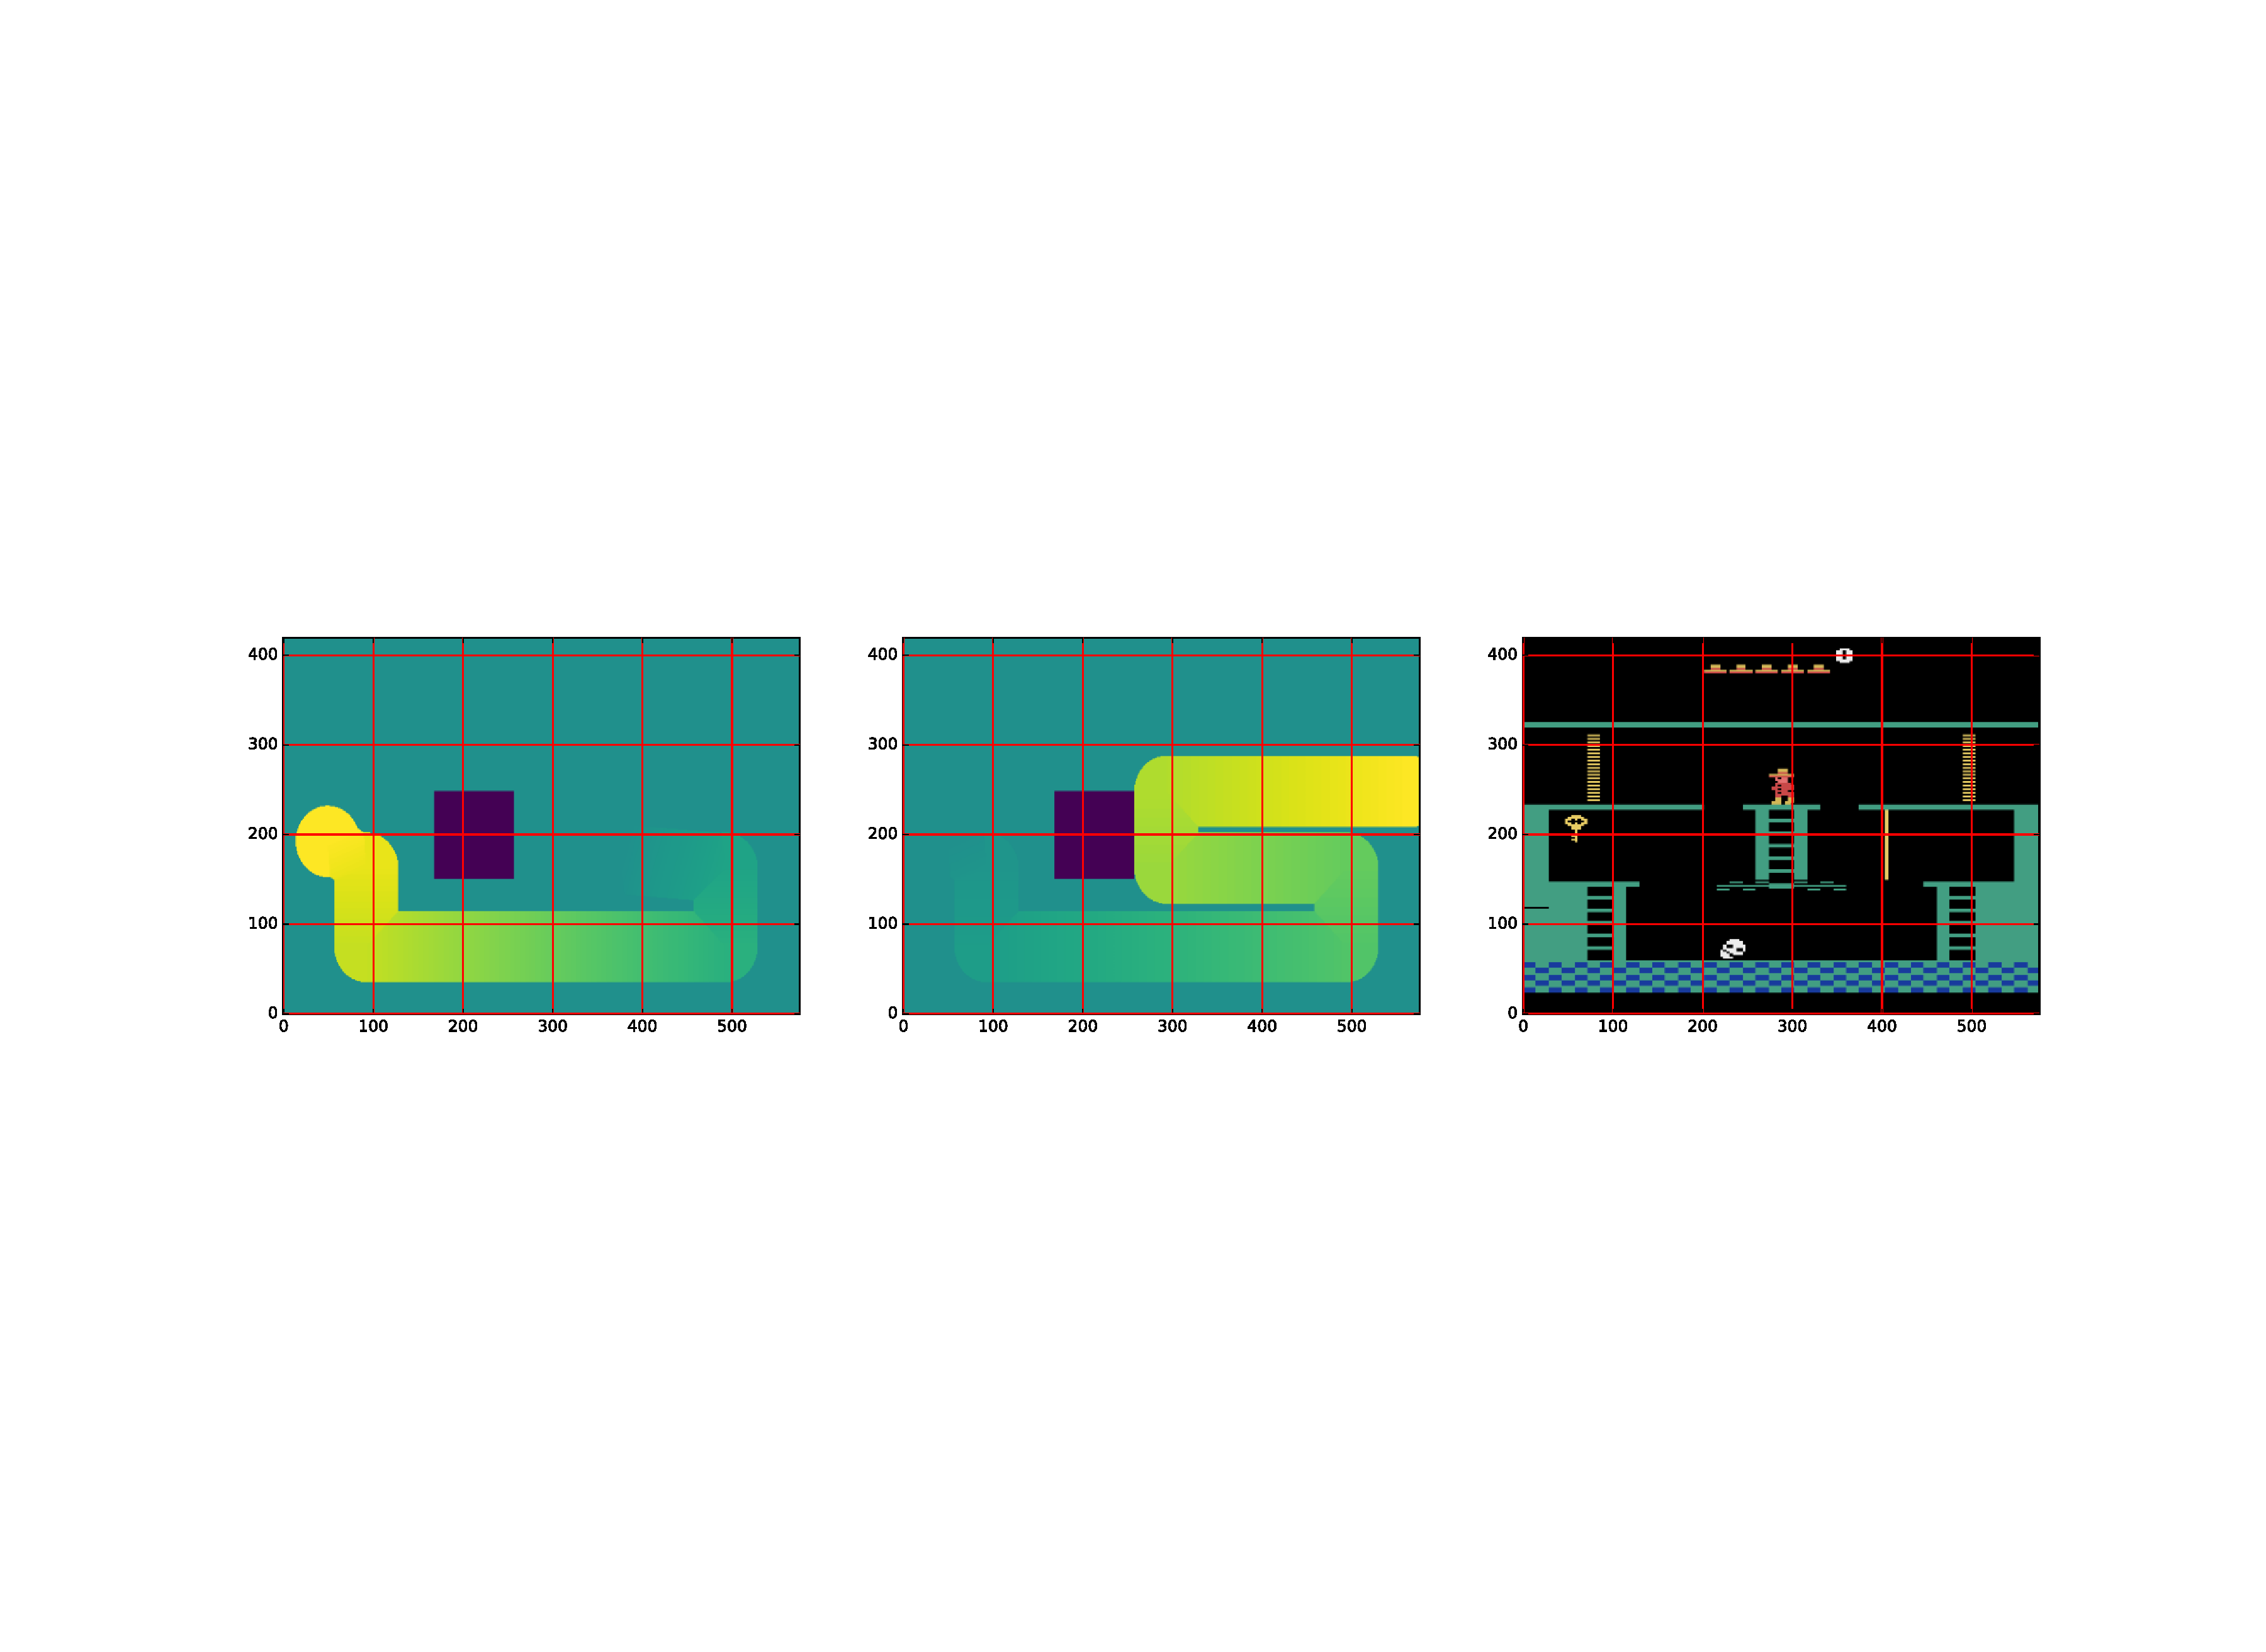
\includegraphics[width=\paperwidth - 1in]{img/shaping.pdf}}
\end{center}
\caption{The shaping potential field used, before and after grabbing the
key.\label{fig:shaping}}
\end{figure}
\begin{equation}
  t_1 = \frac{v_{x_2}(y_1-y_2) - v_{y_2}(x_1-x_2)}{v_{y_2}v_{x_1} - v_{x_2}v_{y_1}}
\end{equation}
\section{Planning}
\subsection{\acl{IW}(1)}
\subsection{\acl{IW}(3) on location}
\subsection{\acl{IW}(3) on location with heuristic}
\section{Learning}
\subsection{Shaped tabular Sarsa}
\subsection{Task by task \acs{DQN}}
\subsection{Tabular Sarsa combined with planning}

%%% Local Variables: 
%%% mode: latex
%%% TeX-master: "../report"
%%% End: 